
% Default to the notebook output style

    


% Inherit from the specified cell style.




    
\documentclass[float=false,crop=false]{standalone}

    
    
\usepackage{../myipy2tex}  % NOTE WE ARE ASSSUMING THE STYLE FILE TO BE ONE FOLDER ABOVE
\usepackage{../myipy2tex_custom}  % YOUR FURTHER CUSTOM STYLES FOR IPYTHON TO LATEX

% if you need to cross reference to any raw tex file from this resultant tex file you  need to refer them here..
% it is not needed when you compile main.tex but make sure the labels are unique
\ifstandalone
\usepackage[numbers]{natbib}
\usepackage{tikz}      % some times raw tikz needed in notebook also..
\usepackage{pgfplots}  % and so is pgfplots
\bibliographystyle{abbrvnat}
\usepackage{xr-hyper} % Needed for external references
    \externaldocument{29_appendix}
    \externaldocument{29_MLE_Regression_Main} 
\title{Hypothesis Testing}
\fi




    


    


    \begin{document}
    
    
    \maketitle
    
    

    
    \section{Applying derivatives to analyze
functions}\label{applying-derivatives-to-analyze-functions}

\subsection{Introduction}\label{introduction}

Inspired from \href{https://youtu.be/lDY9JcFaRd4}{this} video from Khan
Academy.

Here we will have a quick glance on the basics of finding maxima and
minima of a given function.

Maxima - plural of maximum Minima - plural of minimum \([a,b]\) - closed
interval - includes a and b \((a,b)\) - open interval - excludes a and b

\subsection{Critical Points}\label{critical-points}

Given a function \(f(x)\),
% remove input part of cells with tag to_remove
    %((- if cell.metadata.hide_input -))% remove input part of cells with tag to_remove
    %((- if cell.metadata.hide_input -))
    \begin{center}
    \adjustimage{max size={0.9\linewidth}{0.9\paperheight},min size={0.5\linewidth}{!}}{29_appendix_2_files/29_appendix_2_2_0.png}
    \end{center}
    { \hspace*{\fill} \\}
    
    \begin{enumerate}
\def\labelenumi{\arabic{enumi}.}
\tightlist
\item
  There could be a \textbf{global maximum and a minimum} point. Global
  in the sense, inside the \emph{interval}, it is the maximum or minimum
  out of all peaks or valleys.
\item
  There are areas, which are \textbf{local maximum or minium} around
  those areas. There could more than one local maximum or minimum points
  within the interval.
\item
  The slopes at these points are 0 or also \emph{undefined} (sharp
  turn), that is \(f'(x) = 0\) at these points. All these points are
  called \textbf{critical points}.
\item
  Suppose the interval is {[}a,b{]}. Then the \textbf{end points} are
  \(a\) and \(b\) are not critical points, because anyway \(f'(a)\) and
  \(f'(b)\) would be 0 or undefined.\\
\item
  Not all critcal points, which have slope 0, becomes a global or local
  maximum or minimum point. It could have just flattened.
\end{enumerate}

    \subsection{Decreasing or Increasing
Interval}\label{decreasing-or-increasing-interval}

    Inspired from \href{https://youtu.be/KblYjo1Ijws}{this} video from Khan
Academy.

    \paragraph{Decreasing interval}\label{decreasing-interval}

Suppose \(f(x) = x^5(x - 3)\). Below is how the function looks like. We
need to find the interval within which the function is decreasing. Just
by eyeballing, we could know that the green area is where the function
is decreasing, but we are not clear of the exact intervals. This would
could find mathematically.
% remove input part of cells with tag to_remove
    %((- if cell.metadata.hide_input -))% remove input part of cells with tag to_remove
    %((- if cell.metadata.hide_input -))
    \begin{center}
    \adjustimage{max size={0.9\linewidth}{0.9\paperheight},min size={0.5\linewidth}{!}}{29_appendix_2_files/29_appendix_2_8_0.png}
    \end{center}
    { \hspace*{\fill} \\}
    
    Note that, any tangent line drawn on the curve in the green area will
have a negative slope as shown by a blue line. This means, \(f'(x) < 0\)
in those areas. This is the clue. Finding the derivatives, we get

\[
\begin{aligned}
f'(x) = 6x^5 - 15x^4 \\
f'(x) < 0 \implies (6x^5 - 15x^4) < 0 \implies (3x^4)(2x-5) < 0 \\
\end{aligned}
\]

But \(3x^4 >0\) always for any x due to even power, so only possibility
should be \((2x-5) < 0\) or \(x < 2.5\). This means the exact interval
where function is decreasing is \(-\infty < x < 2.5\). Below is the
python implementation of the curve with tangent.
% remove input part of cells with tag to_remove
    %((- if cell.metadata.hide_input -))
    \begin{center}
    \adjustimage{max size={0.9\linewidth}{0.9\paperheight},min size={0.5\linewidth}{!}}{29_appendix_2_files/29_appendix_2_10_0.png}
    \end{center}
    { \hspace*{\fill} \\}
    
    Similarly we could also see where \(x > 2.5\), the curve is increasing.
Summarizing,
\begin{tcolorbox}[colback=green!5,colframe=green!40!black,title=Decreasing or Increasing Interval]
\begin{itemize}
\item If $f'(x) > 0$, then $f(x)$ is increasing.    
\item If $f'(x) < 0$, then $f(x)$ is decreasing.  
\item If $f'(x) = 0$, then its a critical point unless flat trap or endpoints.
\end{itemize} 
\end{tcolorbox} \label{box:RA01}
    \subsection{Flat Traps}\label{flat-traps}

As said earlier, not all critical points are either global or local
maxima or minima. The flat regions might trick one to thin that is a
maximum or minimum point. This is where, a small test around the
critical point becomes important. Taking a small interval of values
around the point, and depending on if \(f'(x)\) is increasing or
decreasing below and above the point, one could conclude if that
critical point was just a flat or extrema (let us refer all critical
points which qualify as maximum or minimum as extremum). Refer
\href{https://youtu.be/x09FpMmGB4A}{1},
\href{https://youtu.be/-ihDprWkcY8}{2} and practice in same session.

    \subsection{Absolute Minima or Maxima (entire
domain)}\label{absolute-minima-or-maxima-entire-domain}

We already saw a hint to avoid flat traps which we could use to identify
the extremum points. Imagine a function like below \(f(x) = x^2\). Just
by eyeballing we could say, it decreases for interval
\(x = (-\infty,0)\) and increases for \(x = (0, \infty)\). So the
absolute minimum happens at \(x=0\), but how do we prove that
mathematically.
% remove input part of cells with tag to_remove
    %((- if cell.metadata.hide_input -))
    \begin{center}
    \adjustimage{max size={0.9\linewidth}{0.9\paperheight},min size={0.5\linewidth}{!}}{29_appendix_2_files/29_appendix_2_15_0.png}
    \end{center}
    { \hspace*{\fill} \\}
    
    We know when the slope is negative, the function is decreasing, and
increasing if positive. We could just take a value before and after our
critical point, and see if that is the case, to decide if the critical
point is minimum or maximum. Let us first find the critical point for
\(f(x)=x^2\) in the interval \([-\infty, \infty]\). Note, this interval
should either be explicitly or implicity defined before we try assessing
the critical points. Here, we are able to take entire infinite range
because of the ever increasing nature of the function before and after
critical point.

\[
f'(x) = 2x
\]

When \(x < 0\), for eg, \(x=-2\), then \(f'(x) = 2(-2) = -4 < 0\), so
its decreasing.\\
When \(x > 0\), for eg, \(x=2\), then \(f'(x) = 2(2) = 4 > 0\), so its
increasing.

Thus, we infer, before critical point, the given function \(x^2\) is
decreasing, and after critical point, the given function \(x^2\) is
increasing. Thus the critical point should be a minimum. Since this is
in entire domain, this is an absolute minimum point for the function
\(x^2\). Refer \href{https://youtu.be/Xhc7Hens0f8}{1} for another
example where the domain is implicit in the function.

If we get more than 1 critical point within the interval, then simply
taking the maximum of all the \(f(x)\) values at those critical points,
will give absolute or global maximum point.

    \subsection{Concavity}\label{concavity}

It is tedious every time to take values around the first derivative so
let us try an easier method of taking second derivative.

Let \(f(x) = x(x-3)^2\). The function, and its derivatives will look
like below.
% remove input part of cells with tag to_remove
    %((- if cell.metadata.hide_input -))
    \begin{center}
    \adjustimage{max size={0.9\linewidth}{0.9\paperheight},min size={0.5\linewidth}{!}}{29_appendix_2_files/29_appendix_2_18_0.png}
    \end{center}
    { \hspace*{\fill} \\}
    
    By eyeballing, one could see, \(f(x)\) reaches a maximum at \(x = 1\).
Understandly, in 2nd graph, we could observe, that \(f'(x)_{x=1} = 0\).
Note the 2nd derivative in 3rd graph is giving one more information,
that it is negative. That is, \(f''(x)_{x=1} < 0\).

\(f(x)\) reaches a minimum at \(x=3\). Understandly, \(f'(x)_{x=3} = 0\)
again. And \(f''(x)_{x=3} > 0\), that is, its positive, indicating that
the original functino \(f(x)\) is increasing.

\(f(x)\) reaches an inflection point at \(x=2\). It is a point at which
, the first derivative reaches a minimum as seen in 2nd graph. Note at
this point, \(f''(x)_{x=2} = 0\). In terms of original function, it is a
point at which the curve stops being a concave (concave downward) and
becomes a conves (or concave upward).

Thus by observing the 2nd derivative, one could conclude about whether a
critical point is maximum or minimum or inflection. However, there is a
trap, this method is not very rigorous. Refer
\href{https://www.quora.com/How-can-a-second-derivative-be-equal-to-zero-at-a-maximum-Shouldnt-it-always-be-less-than-zero}{1}
which explains about the trap.
\begin{tcolorbox}[colback=green!5,colframe=green!40!black,title=Concavity of given function]
\begin{itemize}
\item If $f''(x) > 0$ at $f'(x)=0$, then $f(x)$ is increasing.    
\item If $f''(x) < 0$ at $f'(x)=0$, then $f(x)$ is decreasing.  
\item If $f''(x) = 0$ and $f'(x) \neq 0$, then its an inflection point. But not always.   
\end{itemize}
\end{tcolorbox} \label{box:RA02}
    \subsection{Surface Plots}\label{surface-plots}

The same concepts could also be directly transferred to 3D plots via
partial derivatives. For eg, for a function \(f(x,y)\), given one of the
variables, say \(x\) is a constant \(k\), a critical point occurs when
\(\dfrac{\partial f(x,y)}{\partial y}\bigg|_{x=k} = 0\). Similarly when
\(y=k\), critical point is expected at
\(\dfrac{\partial f(x,y)}{\partial x}\bigg|_{y=k} = 0\)

    Let us consider an example \(z = f(x,y) = (y - x)^2\). If we plot the
figure, we could already observe that its ever increasing on two
directions and has one valley, where the minimum must be occuring. The
contour is also shown on XY plane, where one could observe the minimum
value occurs along the valley line.
% remove input part of cells with tag to_remove
    %((- if cell.metadata.hide_input -))
    \begin{center}
    \adjustimage{max size={0.9\linewidth}{0.9\paperheight},min size={0.5\linewidth}{!}}{29_appendix_2_files/29_appendix_2_23_0.png}
    \end{center}
    { \hspace*{\fill} \\}
    
    Taking partial derivative with \(x\) as constant,

\[
\dfrac{\partial f(x,y)}{\partial y} = \dfrac{\partial (x-y)^2}{\partial y} = 2(x-y)(-1) = -2(x-y)
\]

Assigning it to 0, we get, \[
-2(x-y) = 0 \implies (x - y) = 0 \implies x = y
\]

In fact that is what we observed in above diagram. The critical points
are in fact a line defined by \(x=y\) denoted by dotted white line
above. Let us observe what happens for other possibility (we could
already observe from graph, that it should result in same output
\(x=y\)), there are no other critical lines. Taking partial derivative
with \(y\) as constant,

\[
\dfrac{\partial f(x,y)}{\partial x} = \dfrac{\partial (x-y)^2}{\partial x} = 2(x-y)(1) = 2(x-y)
\]

Assigning it to 0, we get, \[
2(x-y) = 0 \implies (x - y) = 0 \implies x = y
\]

The same answer. Thus, we are able to mathematically find the critical
point. Remember, the first derivative only tells it could be a critical
point, not already maximum or minimum, that should be done after wards.
In our case, from the graph we got the hint its a minimum, but not yet
mathematically.

    \subsubsection{Second order Trap}\label{second-order-trap}

However, we cannot just directly interpret second order partial
derivatives for \(f(x,y)\) like we did for one variable functions. In
fact that would be inconclusive. Something more is needed.

Let us try. We shall keep \(y\) as constant, say \(y=3\). Taking second
order derivative, w.r.t \(x\)

\[
\dfrac{\partial^2 f(x,y)}{\partial x} = \dfrac{\partial^2 (x-y)^2}{\partial x} = \dfrac{\partial 2(x-y)}{\partial x} = 2 > 0
\]

This should mean, our function \(f(x,y)\) should be increasing, but if
you look at \(y=3\) plane, you could observe that as \(x\) is
increasing, the function decreased. However, if you look at the plane
\(y=-3\), \(f(x,y)\) is indeed seem to be increasing with \(x\). This is
illustrated in Fig \(\ref{fig:RA03}\).

    ~
\begin{figure}\small
\begin{minipage}[b]{.5\linewidth}
\centering
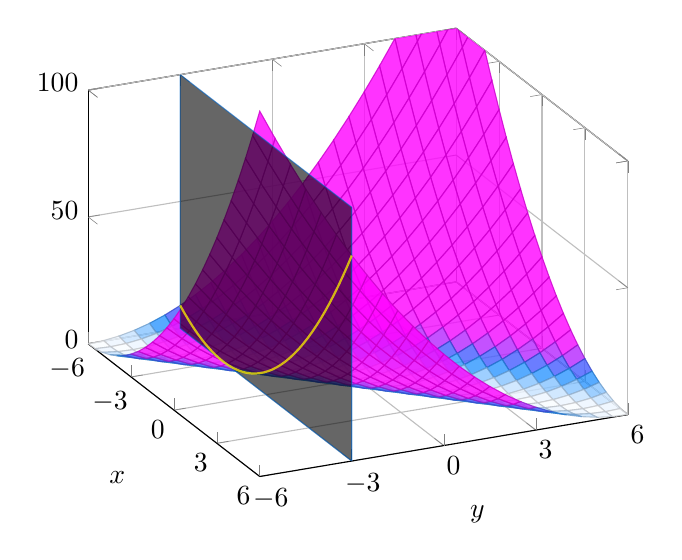
\begin{tikzpicture}
\begin{axis}[
    grid=both,
    xtick={-6,-3,...,6},ytick={-6,-3,...,6}, ztick={0,50,...,100},
    zmin = 0,  zmax = 100,
    xlabel={$x$}, ylabel = {$y$},
    point meta min=0,  point meta max=10,
    colormap/cool,
    view={65}{30}  %tune here to change viewing angle
    ]
    
\def\xc{1} % when x as constant
\def\yc{-3} % when y as constant
\addplot3[surf,shader=faceted, domain=-6:6, opacity=0.8] {(x-y)^2};
\addplot3[surf,mesh/rows=2,black,opacity=0.6] coordinates {(-6,\yc,0) (-6,\yc,100) (6,\yc,0) (6,\yc,100)};
\addplot3+[domain=-6:6,samples=40, samples y=0,  mark=dot,yellow, opacity=0.75,thick]({x},{\yc},{(x-\yc)^2});

\end{axis}
\end{tikzpicture}
\subcaption{f(x,y) increases with $x$ when $y=-3$}\label{fig:RA01}
\end{minipage}%
%
\begin{minipage}[b]{.5\linewidth}
\centering
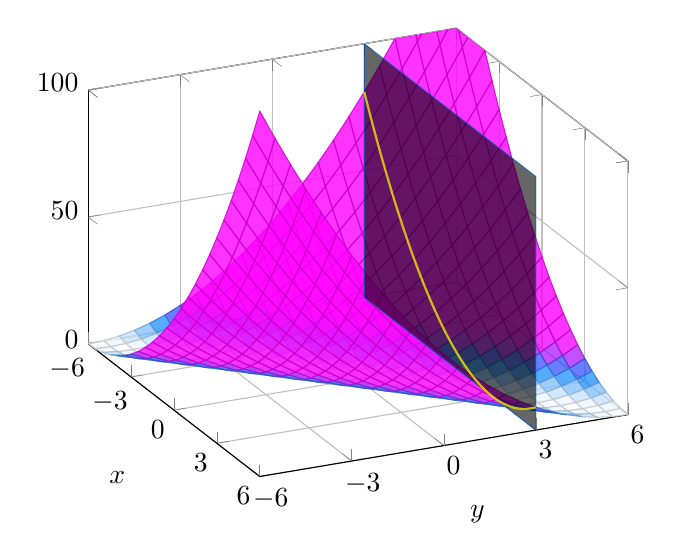
\begin{tikzpicture}
\begin{axis}[
    grid=both,
    xtick={-6,-3,...,6},ytick={-6,-3,...,6}, ztick={0,50,...,100},
    zmin = 0,  zmax = 100,
    xlabel={$x$}, ylabel = {$y$},
    point meta min=0,  point meta max=10,
    colormap/cool,
    view={65}{30}  %tune here to change viewing angle
    ]
    
\def\xc{1} % when x as constant
\def\yc{3} % when y as constant
\addplot3[surf,shader=faceted, domain=-6:6, opacity=0.8] {(x-y)^2};
\addplot3[surf,mesh/rows=2,black,opacity=0.6] coordinates {(-6,\yc,0) (-6,\yc,100) (6,\yc,0) (6,\yc,100)};
\addplot3+[domain=-6:6,samples=40, samples y=0,  mark=dot,yellow, opacity=0.75,thick]({x},{\yc},{(x-\yc)^2});

\end{axis}
\end{tikzpicture}
\subcaption{f(x,y) decreases with $x$ when $y=3$}\label{fig:RA02}
\end{minipage}
\caption{Fig 1: Inconclusivness from $\frac{\partial^2 f(x,y)}{\partial x^2}\bigg|_{y=k}$}  \label{fig:RA03}
\end{figure}
    Similarly, if we try to keep \(x\) as constant, and take partial
derivative w.r.t y,

\[
\dfrac{\partial^2 f(x,y)}{\partial y} = \dfrac{\partial^2 (x-y)^2}{\partial y} = \dfrac{\partial -2(x-y)}{\partial x} = -2(-1) = 2 > 0
\]

Again we see a similar predicament. Observe for both \(x=-3\) and
\(x=3\) as shown in Fig \(\ref{fig:RA06}\).
\begin{figure}\small
\begin{minipage}[b]{.5\linewidth}
\centering
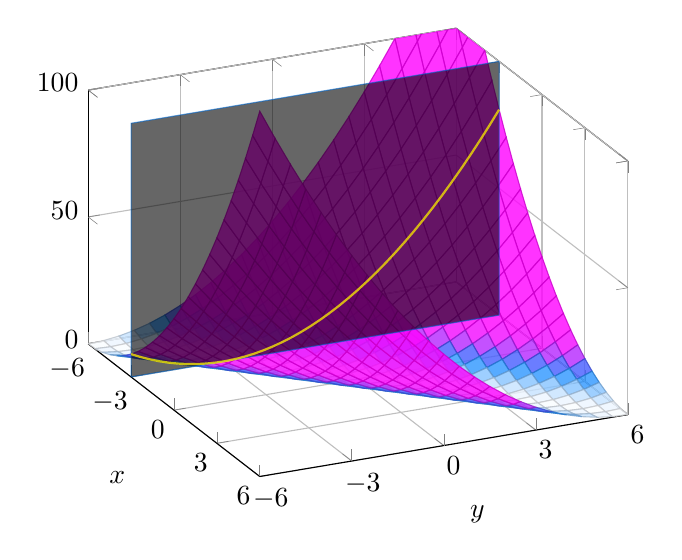
\begin{tikzpicture}
\begin{axis}[
    grid=both,
    xtick={-6,-3,...,6},ytick={-6,-3,...,6}, ztick={0,50,...,100},
    zmin = 0,  zmax = 100,
    xlabel={$x$}, ylabel = {$y$},
    point meta min=0,  point meta max=10,
    colormap/cool,
    view={65}{30}  %tune here to change viewing angle
    ]
    
\def\xc{-3} % when x as constant
\def\yc{-3} % when y as constant
\addplot3[surf,shader=faceted, domain=-6:6, opacity=0.8] {(x-y)^2};
\addplot3[surf,mesh/rows=2,black,opacity=0.6] coordinates {(\xc,-6,0) (\xc,-6,100) (\xc,6,0) (\xc,6,100)};
\addplot3+[domain=-6:6,samples=40, samples y=0,  mark=dot,yellow, opacity=0.75,thick]({\xc},{x},{(\xc-x)^2});

\end{axis}
\end{tikzpicture}
\subcaption{f(x,y) increases with $y$ when $x=-3$}\label{fig:RA04}
\end{minipage}%
%
\begin{minipage}[b]{.5\linewidth}
\centering
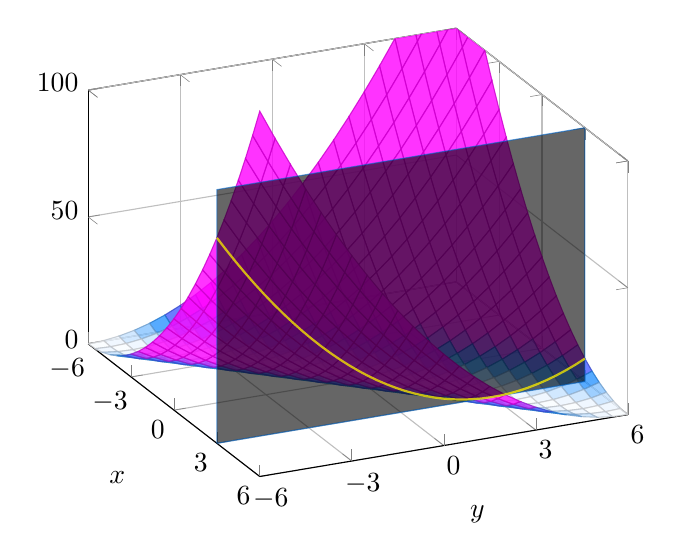
\begin{tikzpicture}
\begin{axis}[
    grid=both,
    xtick={-6,-3,...,6},ytick={-6,-3,...,6}, ztick={0,50,...,100},
    zmin = 0,  zmax = 100,
    xlabel={$x$}, ylabel = {$y$},
    point meta min=0,  point meta max=10,
    colormap/cool,
    view={65}{30}  %tune here to change viewing angle
    ]
    
\def\xc{3} % when x as constant
\def\yc{3} % when y as constant
\addplot3[surf,shader=faceted, domain=-6:6, opacity=0.8] {(x-y)^2};
\addplot3[surf,mesh/rows=2,black,opacity=0.6] coordinates {(\xc,-6,0) (\xc,-6,100) (\xc,6,0) (\xc,6,100)};
\addplot3+[domain=-6:6,samples=40, samples y=0,  mark=dot,yellow, opacity=0.75,thick]({\xc},{x},{(\xc-x)^2});

\end{axis}
\end{tikzpicture}
\subcaption{f(x,y) decreases with $y$ when $x=3$}\label{fig:RA05}
\end{minipage}
\caption{Fig 2: Inconclusivness from $\frac{\partial^2 f(x,y)}{\partial y^2}\bigg|_{x=k}$}  \label{fig:RA06}
\end{figure}
    The inconclusivness is because, there is more to surfaces or two
variable functions \(f(x,y)\) compared to single variable ones. Apart
from minium, maximum they also have saddle points. And the possible
second order partial derivatives are not just two as we saw, but four as
below.

\[\begin{aligned}
f_{xx} = \dfrac{\partial f^2}{\partial x^2} \\
f_{yy} = \dfrac{\partial f^2}{\partial y^2} \\
f_{xy} = \dfrac{\partial f^2}{\partial x \partial y} = \dfrac{\partial f^2}{\partial y \partial x} 
\end{aligned}\]

    Thus in case of surfaces, by making a first order partial
differentiation w.r.t x and y, what we would get could also be a maximum
or minimum or also a saddle point. The method to classify via second
order as I just said, is little bit more involved. We will revisit and
resume in future if needed, but for a quick dip on working that as well
with an example, refer
\href{http://personal.maths.surrey.ac.uk/S.Zelik/teach/calculus/max_min_2var.pdf}{here}


    % Add a bibliography block to the postdoc
    
    
    
    \end{document}
